\documentclass[a4paper]{report}
\pagestyle{headings}
\usepackage{hyperref}
\usepackage{listings}
\usepackage{graphicx}
\lstset{language=bash}
\lstset{numbers=right}
\lstset{breaklines}
\title{Lab Report for Software Engineering course \newline
 Lab 1: Git \& Dev Cloud}
\author{Wang, Chen \\ 16307110064 \\ School of Software\\ Fudan University}
\date{\today}
\bibliographystyle{plain}
\begin{document}
\maketitle

\tableofcontents

\chapter{Background Knowledge of the lab}
\section{Version Control System}
\subsection{The application of VCS}
\par
A component of software configuration management, version control, also known as revision control or source control, is the management of changes to documents, computer programs, large web sites, and other collections of information. Changes are usually identified by a number or letter code, termed the "revision number", "revision level", or simply "revision". For example, an initial set of files is "revision 1". When the first change is made, the resulting set is "revision 2", and so on. Each revision is associated with a timestamp and the person making the change. Revisions can be compared, restored, and with some types of files, merged.

\par
The need for a logical way to organize and control revisions has existed for almost as long as writing has existed, but revision control became much more important, and complicated when the era of computing began. The numbering of book editions and of specification revisions are examples that date back to the print-only era. Today, the most capable (as well as complex) revision control systems are those used in software development, where a team of people may concurrently make changes to the same files.

\par
Version control systems (VCS) most commonly run as stand-alone applications, but revision control is also embedded in various types of software such as word processors and spreadsheets, collaborative web docs and in various content management systems, e.g., Wikipedia's page history. Revision control allows for the ability to revert a document to a previous revision, which is critical for allowing editors to track each other's edits, correct mistakes, and defend against vandalism and spamming in wikis.

\subsection{The general usage of VCS}
\par
In computer software engineering, revision control is any kind of practice that tracks and provides control over changes to source code. Software developers sometimes use revision control software to maintain documentation and configuration files as well as source code.
\par
As teams design, develop and deploy software, it is common for multiple versions of the same software to be deployed in different sites and for the software's developers to be working simultaneously on updates. Bugs or features of the software are often only present in certain versions (because of the fixing of some problems and the introduction of others as the program develops). Therefore, for the purposes of locating and fixing bugs, it is vitally important to be able to retrieve and run different versions of the software to determine in which version(s) the problem occurs. It may also be necessary to develop two versions of the software concurrently: for instance, where one version has bugs fixed, but no new features (branch), while the other version is where new features are worked on (trunk).
\par
At the simplest level, developers could simply retain multiple copies of the different versions of the program, and label them appropriately. This simple approach has been used in many large software projects. While this method can work, it is inefficient as many near-identical copies of the program have to be maintained. This requires a lot of self-discipline on the part of developers and often leads to mistakes. Since the code base is the same, it also requires granting read-write-execute permission to a set of developers, and this adds the pressure of someone managing permissions so that the code base is not compromised, which adds more complexity. Consequently, systems to automate some or all of the revision control process have been developed. This ensures that the majority of management of version control steps is hidden behind the scenes.
\par
Moreover, in software development, legal and business practice and other environments, it has become increasingly common for a single document or snippet of code to be edited by a team, the members of which may be geographically dispersed and may pursue different and even contrary interests. Sophisticated revision control that tracks and accounts for ownership of changes to documents and code may be extremely helpful or even indispensable in such situations.
\par
Revision control may also track changes to configuration files, such as those typically stored in /etc or /usr/local/etc on Unix systems. This gives system administrators another way to easily track changes made and a way to roll back to earlier versions should the need arise.
\subsection{Various tools for VCS}
\subsubsection{Differences between distributive and non-distributive VCS systems}
\par
Distributed version control systems (DVCS) takes a peer-to-peer approach to version control, as opposed to the client–server approach of centralized systems. Distributed revision control synchronizes repositories by exchanging patches from peer to peer. There is no single central version of the codebase; instead, each user has a working copy and the full change history.
\par
Advantages of DVCS (compared with centralized systems) include:
\begin{enumerate}
  \item Allows users to work productively when not connected to a network.
  \item Common operations (such as commits, viewing history, and reverting changes) are faster for DVCS, because there is no need to communicate with a central server. With DVCS, communication is only necessary when sharing changes among other peers.
  \item Allows private work, so users can use their changes even for early drafts they do not want to publish.
  \item Working copies effectively function as remote backups, which avoids relying on one physical machine as a single point of failure.
  \item Allows various development models to be used, such as using development branches or a Commander/Lieutenant model.
  \item Permits centralized control of the "release version" of the project
  \item On FOSS software projects it is much easier to create a project fork from a project that is stalled because of leadership conflicts or design disagreements.
\end{enumerate}
\par
Disadvantages of DVCS (compared with centralized systems) include:
\begin{enumerate}
  \item Initial checkout of a repository is slower as compared to checkout in a centralized version control system, because all branches and revision history are copied to the local machine by default.
  \item The lack of locking mechanisms that is part of most centralized VCS and still plays an important role when it comes to non-mergeable binary files such as graphic assets.
  \item Additional storage required for every user to have a complete copy of the complete codebase history.
\end{enumerate}
\par
Some originally centralized systems now offer some distributed features. For example, Subversion is able to do many operations with no network. Team Foundation Server and Visual Studio Team Services now host centralized and distributed version control repositories via hosting Git.

\section{Git}
\subsection{The feature of Git in comparison to other VCS tools}
\subsubsection{Strong support for non-linear development}
\par
Git supports rapid branching and merging, and includes specific tools for visualizing and navigating a non-linear development history. In Git, a core assumption is that a change will be merged more often than it is written, as it is passed around to various reviewers. In Git, branches are very lightweight: a branch is only a reference to one commit. With its parental commits, the full branch structure can be constructed.
\subsubsection{Distributed development}
Like Darcs, BitKeeper, Mercurial, SVK, Bazaar, and Monotone, Git gives each developer a local copy of the full development history, and changes are copied from one such repository to another. These changes are imported as added development branches and can be merged in the same way as a locally developed branch.
\subsubsection{Compatibility with existent systems and protocols}
Repositories can be published via Hypertext Transfer Protocol (HTTP), File Transfer Protocol (FTP), rsync (removed in Git 2.8.0), or a Git protocol over either a plain socket, or Secure Shell (ssh). Git also has a CVS server emulation, which enables the use of extant CVS clients and IDE plugins to access Git repositories. Subversion and svk repositories can be used directly with git-svn.
\subsubsection{Efficient handling of large projects}
Torvalds has described Git as being very fast and scalable, and performance tests done by Mozilla showed that it was an order of magnitude faster than some version-control systems; fetching version history from a locally stored repository can be one hundred times faster than fetching it from the remote server.
\subsubsection{Cryptographic authentication of history}
The Git history is stored in such a way that the ID of a particular version (a commit in Git terms) depends upon the complete development history leading up to that commit. Once it is published, it is not possible to change the old versions without it being noticed. The structure is similar to a Merkle tree, but with added data at the nodes and leaves. (Mercurial and Monotone also have this property.)
\subsubsection{Toolkit-based design}
Git was designed as a set of programs written in C and several shell scripts that provide wrappers around those programs. Although most of those scripts have since been rewritten in C for speed and portability, the design remains, and it is easy to chain the components together.
\subsubsection{Pluggable merge strategies}
As part of its toolkit design, Git has a well-defined model of an incomplete merge, and it has multiple algorithms for completing it, culminating in telling the user that it is unable to complete the merge automatically and that manual editing is needed.
\subsubsection{Garbage accumulates until collected}
Aborting operations or backing out changes will leave useless dangling objects in the database. These are generally a small fraction of the continuously growing history of wanted objects. Git will automatically perform garbage collection when enough loose objects have been created in the repository. Garbage collection can be called explicitly using \lstinline !git gc --prune! .
\subsubsection{Periodic explicit object packing}
Git stores each newly created object as a separate file. Although individually compressed, this takes a great deal of space and is inefficient. This is solved by the use of packs that store a large number of objects delta-compressed among themselves in one file (or network byte stream) called a packfile. Packs are compressed using the heuristic that files with the same name are probably similar, but do not depend on it for correctness. A corresponding index file is created for each packfile, telling the offset of each object in the packfile. Newly created objects (with newly added history) are still stored as single objects, and periodic repacking is needed to maintain space efficiency. The process of packing the repository can be very computationally costly. By allowing objects to exist in the repository in a loose but quickly generated format, Git allows the costly pack operation to be deferred until later, when time matters less, e.g., the end of a work day. Git does periodic repacking automatically, but manual repacking is also possible with the \lstinline !git gc! command. For data integrity, both the packfile and its index have an SHA-1 checksum inside, and the file name of the packfile also contains an SHA-1 checksum. To check the integrity of a repository, run the \lstinline!git fsck! command.
\subsection{The application of Git}

Git is a distributed version-control system for tracking changes in source code during software development. It is designed for coordinating work among programmers, but it can be used to track changes in any set of files. Its goals include speed, data integrity, and support for distributed, non-linear workflows.
Git was created by Linus Torvalds in 2005 for development of the Linux kernel, with other kernel developers contributing to its initial development. Its current maintainer since 2005 is Junio Hamano.
As with most other distributed version-control systems, and unlike most client–server systems, every Git directory on every computer is a full-fledged repository with complete history and full version-tracking abilities, independent of network access or a central server.
Git is free and open-source software distributed under the terms of the GNU General Public License version 2.

\subsection{The general usage of Git}
\subsubsection{Working with local repositories}
\paragraph{git init}
This command turns a directory into an empty Git repository. This is the first step in creating a repository. After running git init, adding and committing files/directories is possible.
Usage:


\begin{lstlisting}[language=bash]
# change directory to codebase
$ cd /file/path/to/code

# make directory a git repository
$ git init
\end{lstlisting}

\paragraph{git add}
Adds files in the to the staging area for Git. Before a file is available to commit to a repository, the file needs to be added to the Git index (staging area). There are a few different ways to use git add, by adding entire directories, specific files, or all unstaged files.
Usage:
\begin{lstlisting}[language=bash]
$ git add <file or directory name>
\end{lstlisting}
\paragraph{git commit}
Record the changes made to the files to a local repository. For easy reference, each commit has a unique ID.
It’s best practice to include a message with each commit explaining the changes made in a commit. Adding a commit message helps to find a particular change or understanding the changes.
Usage:
\begin{lstlisting}[language=bash]
# Adding a commit with message
$ git commit -m "Commit message in quotes"
\end{lstlisting}

\paragraph{git status}
This command returns the current state of the repository.
\emph{git status} will return the current working branch. If a file is in the staging area, but not committed, it shows with \emph{git status}. Or, if there are no changes it'll return \emph{nothing to commit, working directory clean}.
Usage:
\begin{lstlisting}[language=bash]
$ git status
\end{lstlisting}

\paragraph{git config}
With Git, there are many configurations and settings possible. \emph{git config} is how to assign these settings. Two important settings are user user.name and user.email. These values set what email address and name commits will be from on a local computer. With \emph{git config}, a \emph{--global} flag is used to write the settings to all repositories on a computer. Without a \emph{--global} flag settings will only apply to the current repository that you are currently in.
There are many other variables available to edit in \emph{git config}. From editing color outputs to changing the behavior of \emph{git status}.
Usage:
\begin{lstlisting}[language=bash]
$ git config <setting> <command>
\end{lstlisting}

\paragraph{git branch}
To determine what branch the local repository is on, add a new branch, or delete a branch.
Usage:
\begin{lstlisting}[language=bash]
# Create a new branch
$ git branch <branch_name>

# List all remote or local branches
$ git branch -a

# Delete a branch
$ git branch -d <branch_name>
\end{lstlisting}


\paragraph{git checkout}
To start working in a different branch, use \emph{git checkout} to switch branches.
Usage:
\begin{lstlisting}[language=bash]
# Checkout an existing branch
$ git checkout <branch_name>

# Checkout and create a new branch with that name
$ git checkout -b <new_branch>
\end{lstlisting}

\paragraph{git merge}
Integrate branches together. \emph{git merge} combines the changes from one branch to another branch. For example, merge the changes made in a staging branch into the stable branch.
Usage:
\begin{lstlisting}[language=bash]
# Merge changes into current branch
$ git merge <branch_name>
\end{lstlisting}
\subsubsection{Working with remote repositories}
\paragraph{git remote}
To connect a local repository with a remote repository. A remote repository can have a name set to avoid having to remember the URL of the repository.
Usage:
\begin{lstlisting}[language=bash]
# Add remote repository
$ git remote <command> <remote_name> <remote_URL>

# List named remote repositories
$ git remote -v
\end{lstlisting}

\paragraph{git clone}
To create a local working copy of an existing remote repository, use \emph{git clone} to copy and download the repository to a computer. Cloning is the equivalent of \emph{git init} when working with a remote repository. Git will create a directory locally with all files and repository history.
Usage:
\begin{lstlisting}[language=bash]
$ git clone <remote_URL>
\end{lstlisting}

\paragraph{git pull}
To get the latest version of a repository run \emph{git pull}. This pulls the changes from the remote repository to the local computer.
Usage:
\begin{lstlisting}[language=bash]
$ git pull <branch_name> <remote_URL/remote_name>
\end{lstlisting}


\paragraph{git push}
Sends local commits to the remote repository. \emph{git push} requires two parameters: the remote repository and the branch that the push is for.
Usage:
\begin{lstlisting}[language=bash]
$ git push <remote_URL/remote_name> <branch>

# Push all local branches to remote repository
$ git push -all
\end{lstlisting}

\subsection{The usage of Git in this lab}
In this lab, we are going to utilize Git to get and modify the code created by the teaching assistant, upload them to the server and then finish other consequent operations. Therefore, the critical steps in our lab include
\begin{enumerate}
  \item Clone the code from the Huawei cloud repository;
  \item Commit our changes to the Git system;
  \item Push our commit onto the Huawei cloud repository.
\end{enumerate}
\subsubsection{Clone}
To check out the code from the repository on the Huawei Cloud platform, we ought to navigate to \url{classroom.devcloud.huaweicloud.com}, login via IAM method, enter the project and navigate to the code management section. The Lab1 section is shown in the list allowing us to clone/download the repository from the cloud. As we select the "via HTTPS" method, we get a link enabling us to clone the code from the Git console.
After getting the link, we can clone the code by entering the following the command below:
\begin{lstlisting}[language=bash]
git clone https://codehub.devcloud.huaweicloud.com/2019rjgc_Lab1_xzstudent00300001/Lab1.git
\end{lstlisting}
\par
After cloning the repository without specifying the path to save the contents, we will get the downloaded files in the user folder by default.
\subsubsection{Commit}
After changing the source code, we can view the changes we have made by using the \textbf{git status} command in the git root folder. The changes will be displayed in the command line window. As we confirm the changes we have made, we can commit the changes by input the \textbf{git commit} command to commit the changes. It should be noted that the commit message is required for each commit we have made. A commit successful message will be shown after a successful commit.
\subsubsection{Push}
After committing the specified codes into the local repository, we can push the commits into the cloud repository. If we have made multiple commits, they will be pushed to the cloud in the single push command.
\par
Since we have specified the remote repositories where we pulled the codes from, we will be free from entering the remote address of the repository again. A single \textbf{git push} command will be able to instruct the git system to push all the commits to the remote repository at the Huawei Cloud.
\section{Java EE}
\subsection{The needs and application of Java EE}
Java Platform, Enterprise Edition (Java EE) is the standard in community-driven enterprise software. Java EE is developed using the Java Community Process, with contributions from industry experts, commercial and open source organizations, Java User Groups, and countless individuals. Each release integrates new features that align with industry needs, improves application portability, and increases developer productivity.
\par
Today, Java EE offers a rich enterprise software platform and with over 20 compliant Java EE implementations to choose from.
\par
As stated above, the Java EE platform is designed to help developers create large-scale, multitiered, scalable, reliable, and secure network applications. A shorthand name for such applications is enterprise applications, so called because these applications are designed to solve the problems encountered by large enterprises. Enterprise applications are not only useful for large corporations, agencies, and governments, however. The benefits of an enterprise application are helpful, even essential, for individual developers and small organizations in an increasingly networked world.
\par
The features that make enterprise applications powerful, like security and reliability, often make these applications complex. The Java EE platform reduces the complexity of enterprise application development by providing a development model, API, and runtime environment that allow developers to concentrate on functionality.
\subsection{Common frameworks of Java EE}
According to some online materials, I have discovered that there are a list of Spring framework that are most commonly used by enterprises across the world. Ordered by popularity, these frameworks are:
\begin{enumerate}
  \item \textbf{Spring MVC.} Old but gold, Spring MVC is still ahead of the curve after more than a decade since its first release. After its expansion to embrace complete MVC framework, Spring kept on evolving adopting changes and turned into a full-scale Java framework for Internet-facing applications, offering software engineers a powerful toolkit for web application development and application configuration as well as for security projects.
  \item \textbf{Struts 2.} To elaborate even more on existing Java frameworks that are widely used by modern software engineers, we decided to refer to the successor of Apache’s Struts 1, Struts 2. This Java framework is quite a find for engineers who work with building contemporary Java EE web apps.
  \item \textbf{Hibernate.} Although not on RebelLabs’ list either, it is worth mentioning Hibernate when debating the best Java framework. This mapping Java framework cracks object-relational impedance mismatch issues by substituting persisting DB accesses high-level object handling functions.
  \item \textbf{JSF.} Being a part of Java EE, JavaServer Faces is supported by Oracle. Although this one is not the best frameworks for speedy Java development, it is easy to utilize because of great documentation provided by Oracle.
  \item \textbf{Vaadin.} Using GWT for rendering the end web page, Vaadin became one of the uber popular frameworks modern developers choose when creating applications for business. Utilizing a well-known component-based approach, Vaadin takes the burden off developer’s shoulder by communicating the changes made to the browser.
  \item \textbf{Google Web Toolkit.} GWT is an another free Java framework allowing coders to create and optimize sophisticated web-based apps.
  \item \textbf{Grails.} This particular web framework is regarded as a dynamic tool enhancing engineers’ productivity due to its opinionated APIs, sensible defaults, as well as its convention-over-configuration paradigm. Seamless Java integration makes this particular framework one of the top choices for plenty of programmers worldwide.
\end{enumerate}
\section{Spring Boot}
\subsection{The feature of Spring Boot in comparison to other Java EE frameworks}
Spring Boot makes it easy to create stand-alone, production-grade Spring based Applications that we can ``just run''.
\par
The designers of Spring Boot take an opinionated view of the Spring platform and third-party libraries so we can get started with minimum fuss. Most Spring Boot applications need very little Spring configuration.
\par
Specifically, Spring Boot has the following features:
\begin{enumerate}
  \item Create stand-alone Spring applications;
  \item Embed Tomcat, Jetty or Undertow directly (no need to deploy WAR files);
  \item Provide opinionated ``starter'' dependencies to simplify your build configuration;
  \item Automatically configure Spring and 3rd party libraries whenever possible;
  \item Provide production-ready features such as metrics, health checks and externalized configuration;
  \item Absolutely no code generation and no requirement for XML configuration.
\end{enumerate}
\subsection{The usage of Spring Boot in this lab}
The main part of the project is based on the Spring Boot framework. In the framework, we have reset the Spring Application run class to be Lab1Applacation, then the controller of the Spring Boot Application is reset to Hello Controller class, whose mapping is requested at ``/Hello''. The index method under the Hello Controller class is quite simple, returning a String showing the name and student ID, which each student should change to their own information.
\par
In addition to these properties, the Spring Boot application should specify a assigned port number, indicating that it will not run on the default port. The reason for this is that a couple of students are running their applications on the same server, who has a unique IP address. However, if all of them use the same port number, part of them won't be able to start the service due to port resource conflict. Assigning each student a unique port number enables them to start the service concurrently.
\section{Classroom platform of Huawei Cloud}
\subsection{The functionalities of Huawei Cloud}
HUAWEI CLOUD, the cloud service brand of the Huawei marquee, packages the 30-plus years of expertise in ICT infrastructure products and solutions so customers can build what they need into their profile with building block-like ease. The brand is committed to providing stable, secure, reliable, and sustainable cloud services to help organizations of all sizes grow in the intelligent world. Complementing the already impressive offerings, the Inclusive AI strategy from HUAWE CLOUD allows everyone to get what they need at an affordable price point, efficiently make easy use of cutting-edge technologies, and rest assured that their profile remains fully secure throughout the entire life cycle.
\par
HUAWEI CLOUD provides a powerful computing platform and easy-to-use development platform to support Huawei's full-stack, all-scenario AI strategy. At HUAWEI CONNECT 2018, HUAWEI CLOUD released its one-stop AI development platform ModelArts, AI vision application development platform HiLens, and quantum computing simulator and programming framework HiQ. Huawei also set up its AI Developer Enablement Program to foster collaboration with developers, partners, universities, and research institutions, with the ultimate goal of making AI more inclusive.
\subsection{The functions of Huawei Cloud used in this lab}
Within the scope of this lab, we are going to finish all periods of the life cycle of our project on the Huawei Cloud platform.
\par
First of all, the start-up codes that the teaching assistants have prepared are put on the Code Management section on the cloud platform. We ought to clone the codes from the repository to our local desktop to make modifications. After proper modification, we need to commit our changes and push them to the remote repository on the Huawei Cloud. After the codes of our version are well-prepared, we can deploy the project with the help of the modularized steps of the Huawei Cloud in the deploy section. Each of us is assigned a server machine account, the system being Linux CentOS. After the steps of installing the JDK, configuring the Spring Boot environments and choosing the project source files, our project can be started.
\par
During the period of the service running, we should visit our server via the IP address and port number and will be able to see the hello page if our service is started successfully, the Spring Boot service listens on the specified port and the launcher class is invoked successfully.
\section{Life cycle in software engineering}
\subsection{The meaning of life cycle in software engineering}
The systems development life cycle (SDLC), also referred to as the application development life-cycle, is a term used in systems engineering, information systems and software engineering to describe a process for planning, creating, testing, and deploying an information system. The systems development life cycle concept applies to a range of hardware and software configurations, as a system can be composed of hardware only, software only, or a combination of both. There are usually six stages in this cycle: analysis, design, development and testing, implementation, documentation, and evaluation.
\par
A systems development life cycle is composed of a number of clearly defined and distinct work phases which are used by systems engineers and systems developers to plan for, design, build, test, and deliver information systems. Like anything that is manufactured on an assembly line, an SDLC aims to produce high-quality systems that meet or exceed customer expectations, based on customer requirements, by delivering systems which move through each clearly defined phase, within scheduled time frames and cost estimates. Computer systems are complex and often (especially with the recent rise of service-oriented architecture) link multiple traditional systems potentially supplied by different software vendors. To manage this level of complexity, a number of SDLC models or methodologies have been created, such as waterfall, spiral, Agile software development, rapid prototyping, incremental, and synchronize and stabilize.
\par
SDLC can be described along a spectrum of agile to iterative to sequential methodologies. Agile methodologies, such as XP and Scrum, focus on lightweight processes which allow for rapid changes (without necessarily following the pattern of SDLC approach) along the development cycle. Iterative methodologies, such as Rational Unified Process and dynamic systems development method, focus on limited project scope and expanding or improving products by multiple iterations. Sequential or big-design-up-front (BDUF) models, such as waterfall, focus on complete and correct planning to guide large projects and risks to successful and predictable results. Other models, such as anamorphic development, tend to focus on a form of development that is guided by project scope and adaptive iterations of feature development.
\subsection{The life cycle displayed in this lab}
In this lab, we can see the full period of the life cycle in a project in software engineering. Specifically, the steps are displayed in the following ways:
\begin{enumerate}
  \item \textbf{Planning.} The platform to place the codes and accomplish the management work, the framework to accomplish the back end and the front end of the server, the server system environment, the displaying user interface and the way to hand in the works are already worked out by the teaching assistants.
  \item \textbf{Analysis.} The teaching assistants should consider how long the time limit should be given to the students, how detailed the documentation should be written and whether the difficulty is suitable for the students.
  \item \textbf{Design.} After analysis, the teaching assistants should make appropriate frameworks, make sure that they can be started successfully, the interfaces are clearly specified and finally, place the codes on the Huawei Cloud platform.
  \item \textbf{Implementation.} The students should follow the instructions of the teaching assistants and implement the concrete methods. Here specifically, we need only to modify a String and a port number.
  \item \textbf{Maintenance.} Here this version of the Lab requires no maintenance after submission.
\end{enumerate}
\chapter{Steps of accomplishing this Lab}
\section{Git operations}
\subsection{Log in}
First of all, we should log in to the Classroom platform at \url{classroom.devcloud.huaweicloud.com/}, log in via \emph{IAM Log in} with the assigned account name and set password. Then we can select the homework section to enter the homework in the software engineering class.
\subsection{DevCloud console}
Then we need to select the Lab1 in the homework list, create a Dev Cloud project from the teacher's template. After waiting for the system to finish creating the project, we can enter the Dev Cloud console. 
\subsection{Code Management}
\subsubsection{Code Repository}
Then we can select the code management section to view the repository for this Lab. In order to clone the code from the remote repository to the local machine, we need to select the \emph{HTTPS} visiting method and copy the address of the repository.
\subsubsection{Clone the repository}
Enter the following code in the local terminal, followed by the account name and password to clone the repository to the local machine. 
\begin{lstlisting}[language=bash]
git clone https://codehub.devcloud.huaweicloud.com/2019rjgc_Lab1_xzstudent00300001/Lab1.git
\end{lstlisting}
\begin{figure}
  \centering
  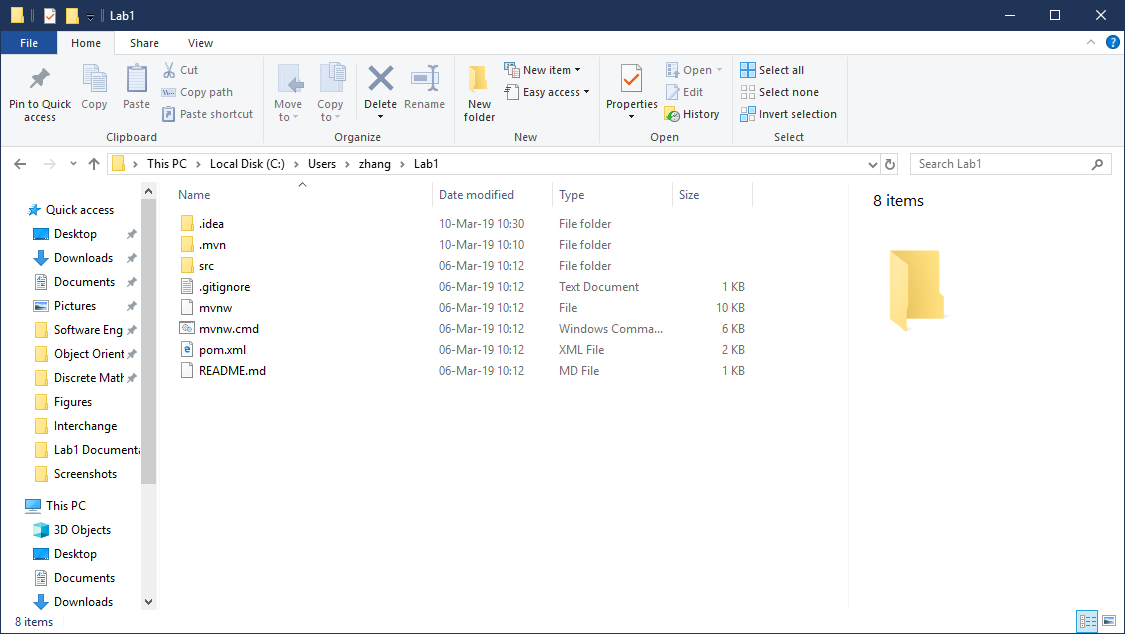
\includegraphics[width=12cm]{Figures/Cloned.png}
  \caption{Clone the repository to the local machine}\label{1}
\end{figure}
After cloning the repository without specifying the path to save the contents, we will get the downloaded files in the user folder by default. The cloned files are like the figure shown in (Figure \ref{1})
\subsubsection{Modify the source code}
There are two places that we need to modify the source code. In the file \emph{\textbackslash src\textbackslash main\textbackslash java\textbackslash fudan\textbackslash se\textbackslash lab1\textbackslash Lab1Application.java}, I need to modify the String to \emph{``Hello, Name: Wang Chen, Id: 16307110064''}; and in the file \emph{\textbackslash src\textbackslash main \textbackslash resources\textbackslash application.properties}, here we need to modify the port number to the specified number. The modified files are shown as the following pictures Figure \ref{2} and Figure \ref{3}.
\begin{figure}
  \centering
  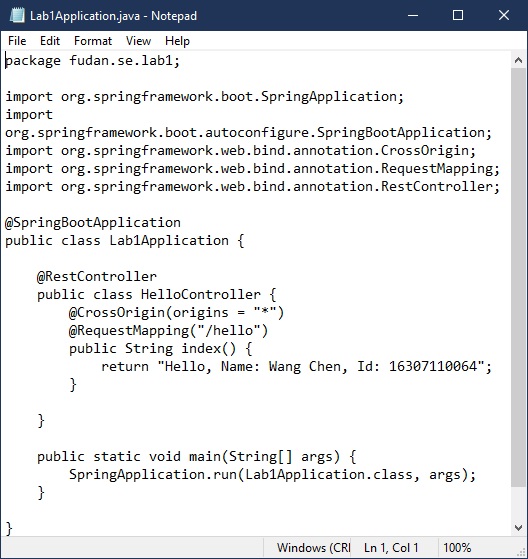
\includegraphics[width=12cm]{Figures/Source.png}
  \caption{Changes of the string}\label{2}
\end{figure}
\begin{figure}
  \centering
  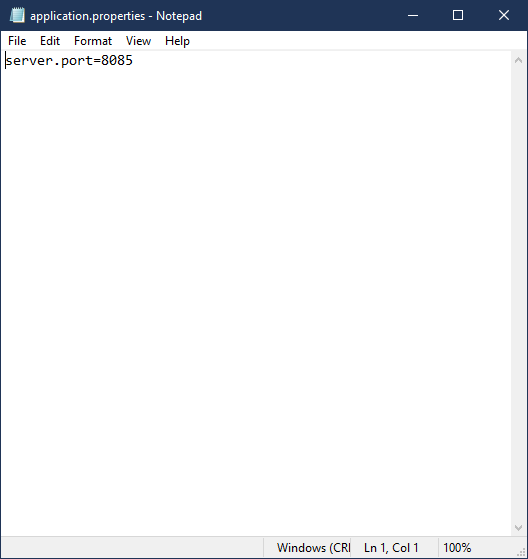
\includegraphics[width=12cm]{Figures/Capture3.png}
  \caption{Changes of the port number}\label{3}
\end{figure}
\subsubsection{View repository status}
After I have modified the codes, I should navigate to the repository folder and view the status of the repository. In the bash shell terminal, I input the commands \emph{cd Lab1} and \emph{git status} specifically. Then the modified file is shown in red color. In the screenshot commit operation, I only changed the first file, leaving the next file's change to the next commit. The status of this change is shown in the Figure \ref{4} below.
\begin{figure}
  \centering
  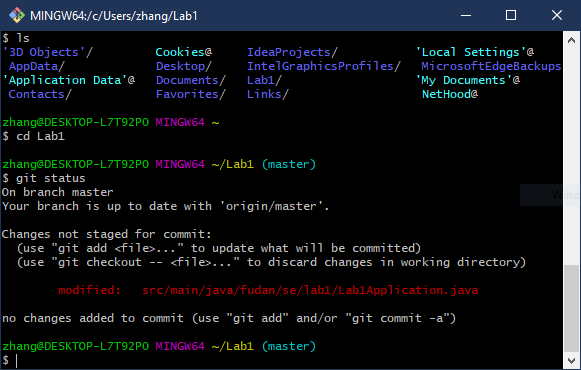
\includegraphics[width=12cm]{Figures/Capture1.png}
  \caption{Status of the git folder}\label{4}
\end{figure}
\subsubsection{Commit changes}
The command \emph{git add .} under the working folder adds the changes to the local cache area of the Git. Afterwards, the \emph{git commit . -m ``~commit message''} command will commit the changes, where the commit message is specified to be \emph{``update name and id''}. The commit result is shown as the Figure \ref{5} below.
\begin{figure}
  \centering
  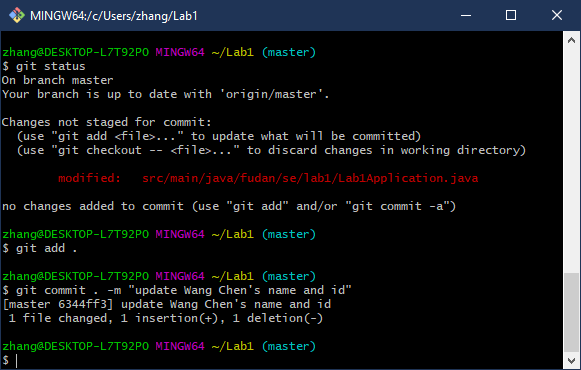
\includegraphics[width=12cm]{Figures/Capture2.png}
  \caption{Result of the \emph{git commit} command}\label{5}
\end{figure}
\subsubsection{Push commits}
As we finish making changes and committing them, we can use the \emph{git push} command to push the changes to the remote repository. The result of the \emph{push} command is shown as the Figure \ref{6} below.
\begin{figure}
  \centering
  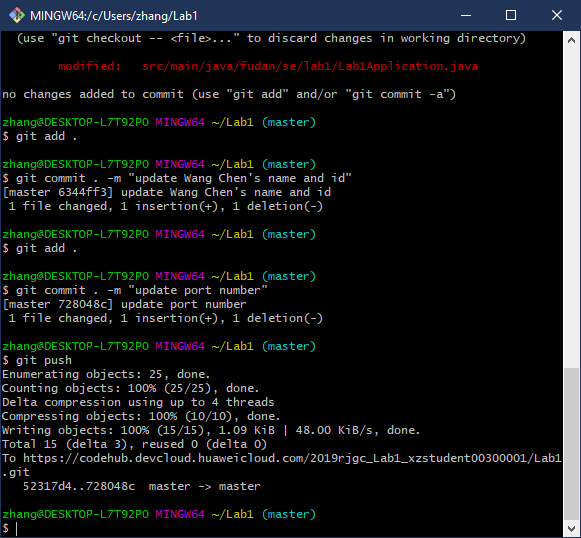
\includegraphics[width=12cm]{Figures/Capture5.png}
  \caption{Result of the \emph{git push} command}\label{6}
\end{figure}
\section{Spring Boot framework construction}
Going back to the Dev Cloud workstation console, we can deploy the project we have just finished editing. Selecting the Build release section and the compile construction subsection, we can create a new task with our student ID and name being the name of the task. Then we need to select the source code from the code management repository and the master branch. After selecting the \emph{Maven Template} option, we can create a new task. As we finish the deploy process, we can see a \emph{Finished Success} prompt, indicating that the deploy process is finished. The result of my deploy is shown in the Figure \ref{7} above.
\begin{figure}
  \centering
  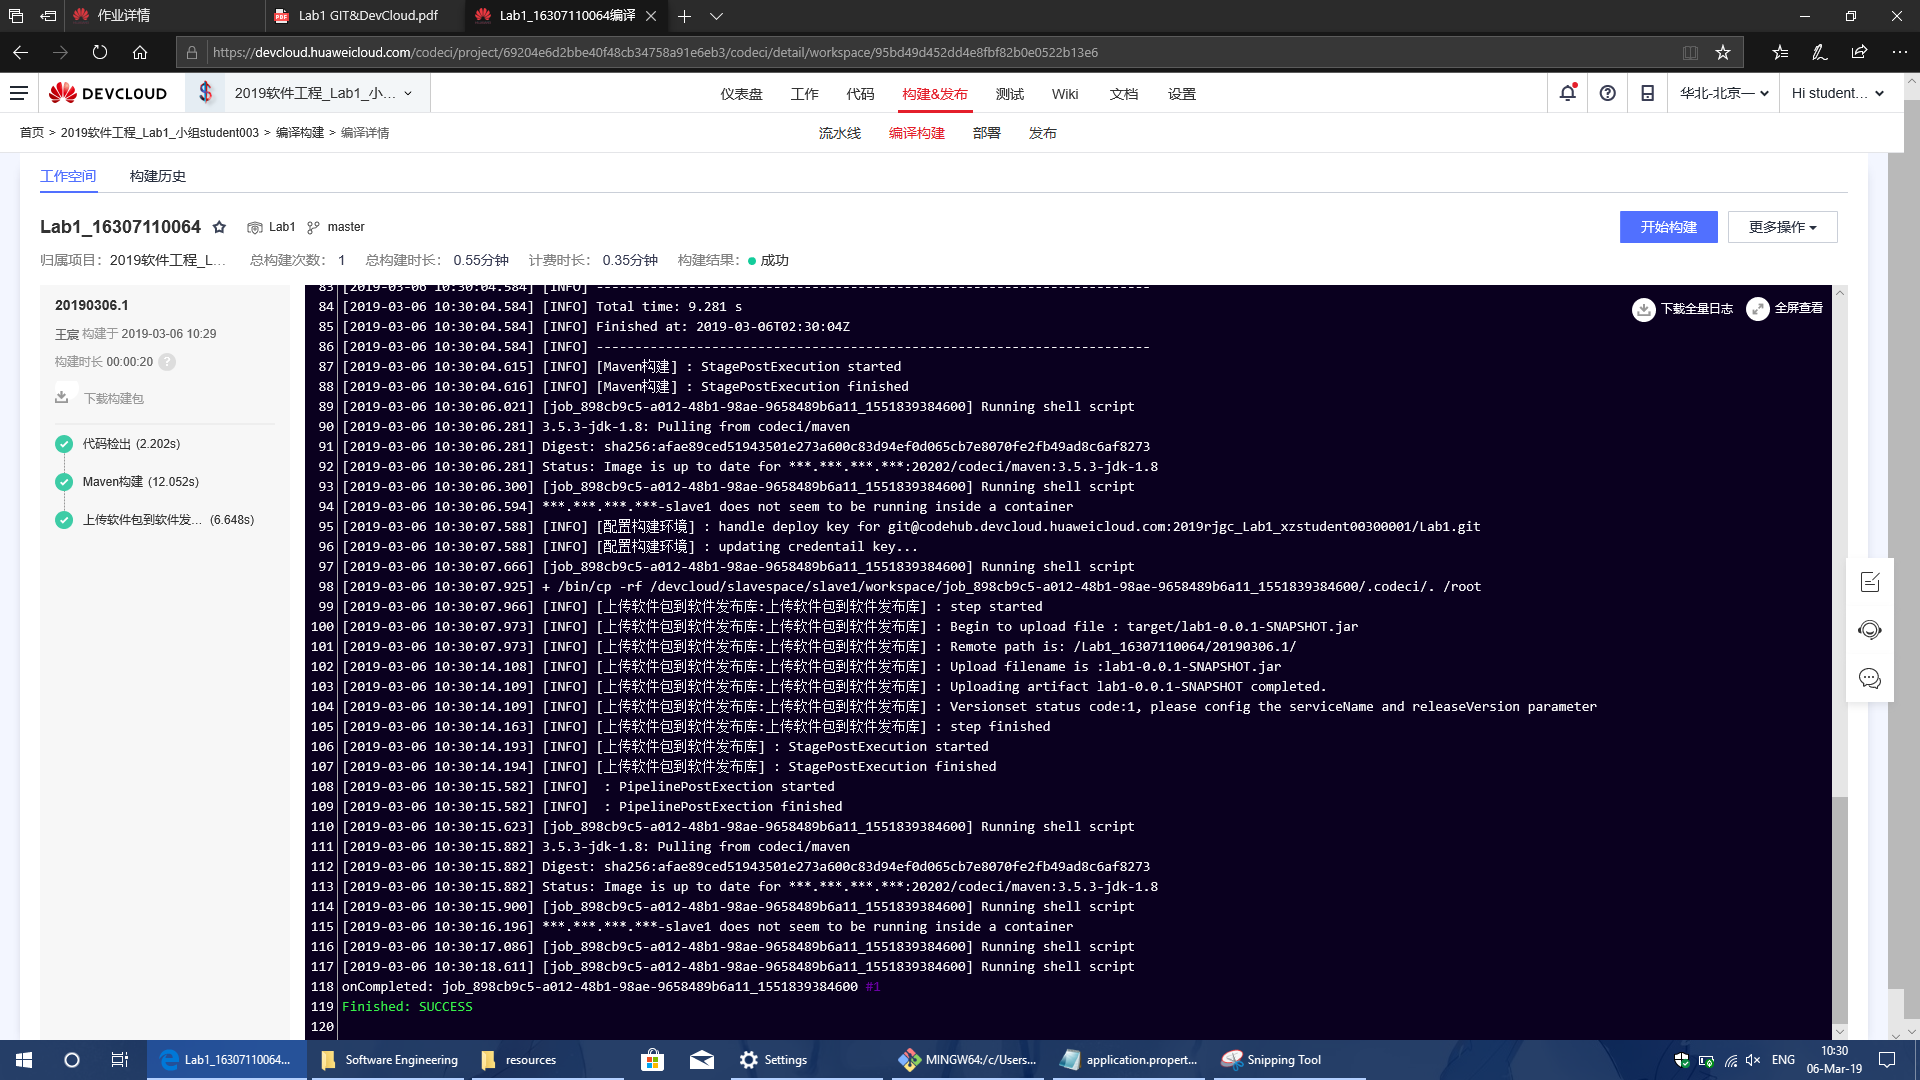
\includegraphics[width=12cm]{Figures/Screenshot(33).png}
  \caption{Result of the first deploy process}\label{7}
\end{figure}
\section{Executions on the Spring Boot framework}
\subsection{Create a new task}
We should create a new task and name the task with our student ID and name. In the next step, we should choose the Spring Boot deployment and go down to the next step.
\subsection{Adjust the deploy sequence}
We should drag the ``Stop Spring Boot service'' to the end of the list and remove the ``URL health test'' method. After removing, we ought to add a new service called ``Pending execution'' between ``Start Spring Boot Service'' and ``Stop Spring Boot Service''. The result of the adjusted deploy sequence is shown as the Figure \ref{8} below.
\begin{figure}
  \centering
  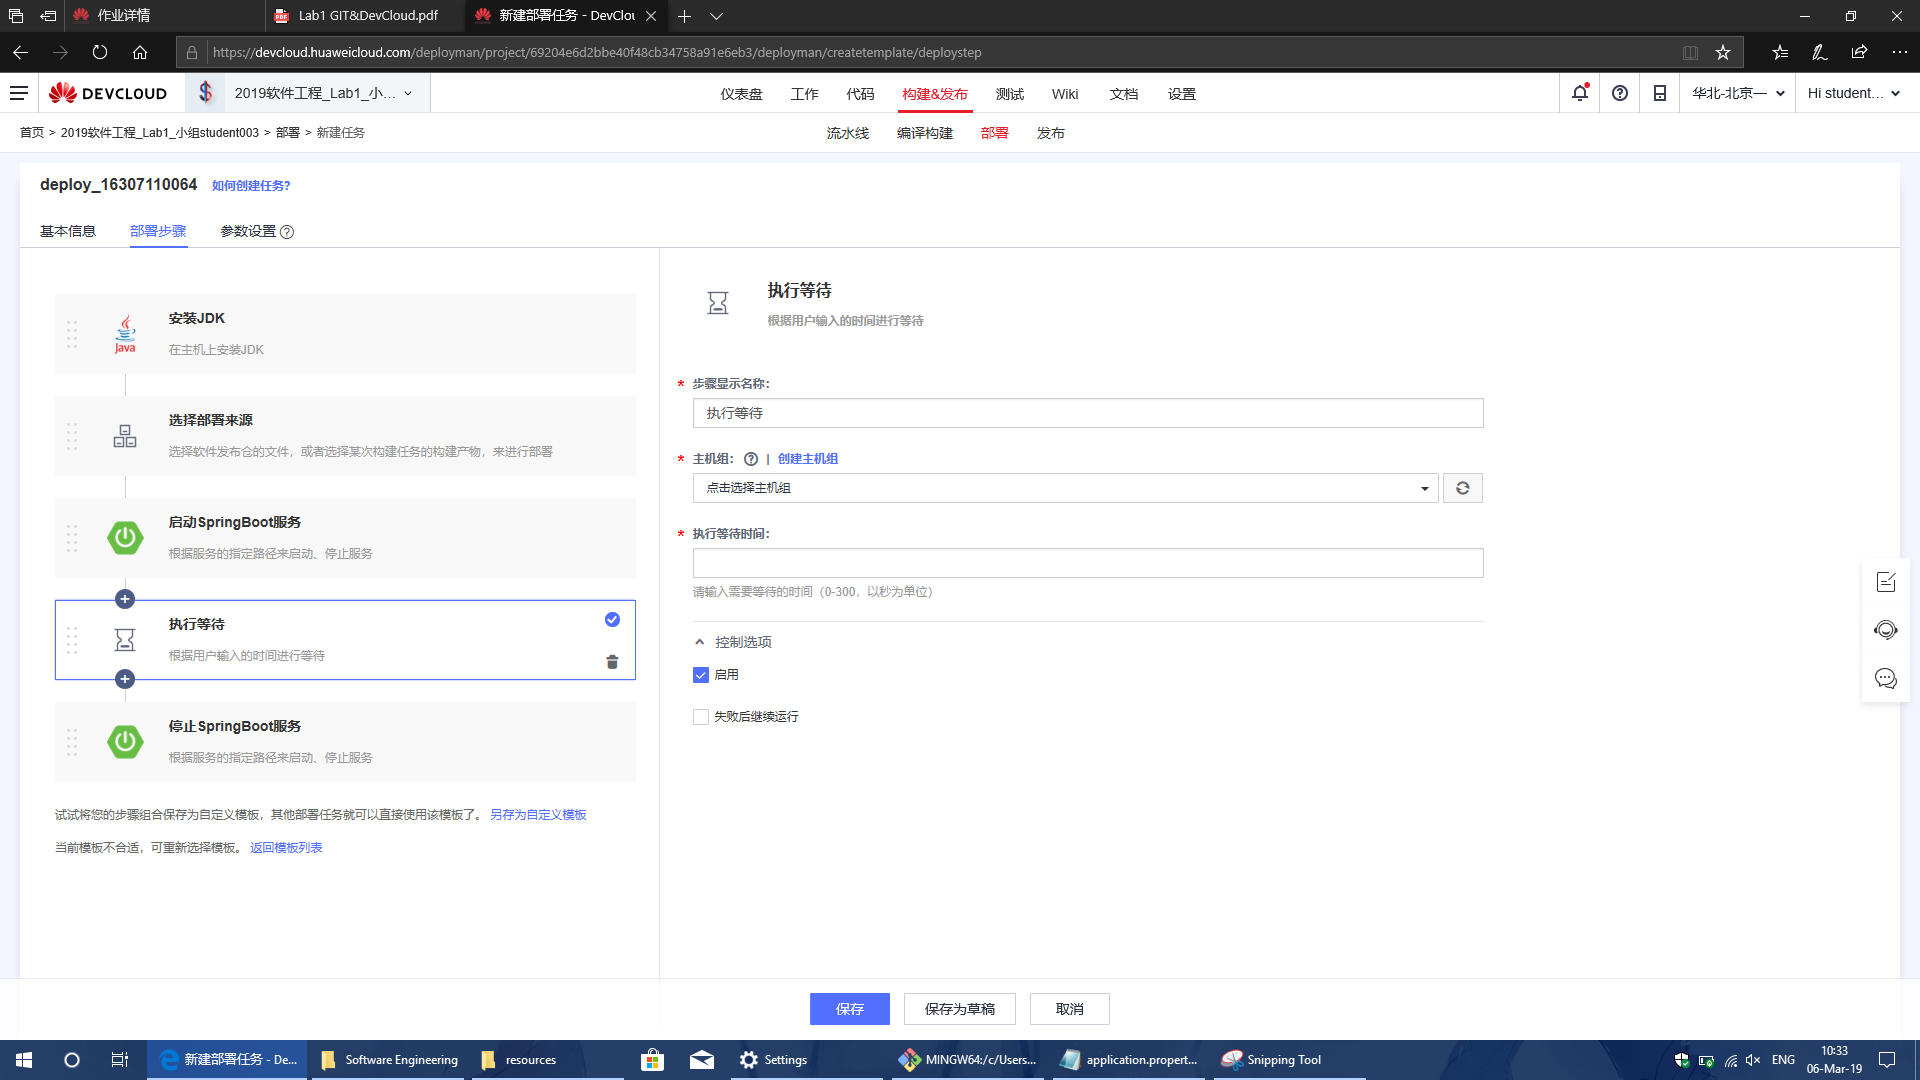
\includegraphics[width=12cm]{Figures/Screenshot(34).png}
  \caption{Result of the adjusted deploy sequence}\label{8}
\end{figure}
\subsection{Configure and install the JDK}
We should create a machine group in the configuring JDK part and create a new host according to the given information. Then we can install the JDK at \emph{/usr/local/jdk}.
\subsection{Choose deployment origin}
In the choosing deployment origin section, we can select the host we have just created and the task we have deployed in the previous part, downloading it to the \emph{/usr/local} path. The result of the configured deployment origin is shown as the Figure \ref{9} below.
\begin{figure}
  \centering
  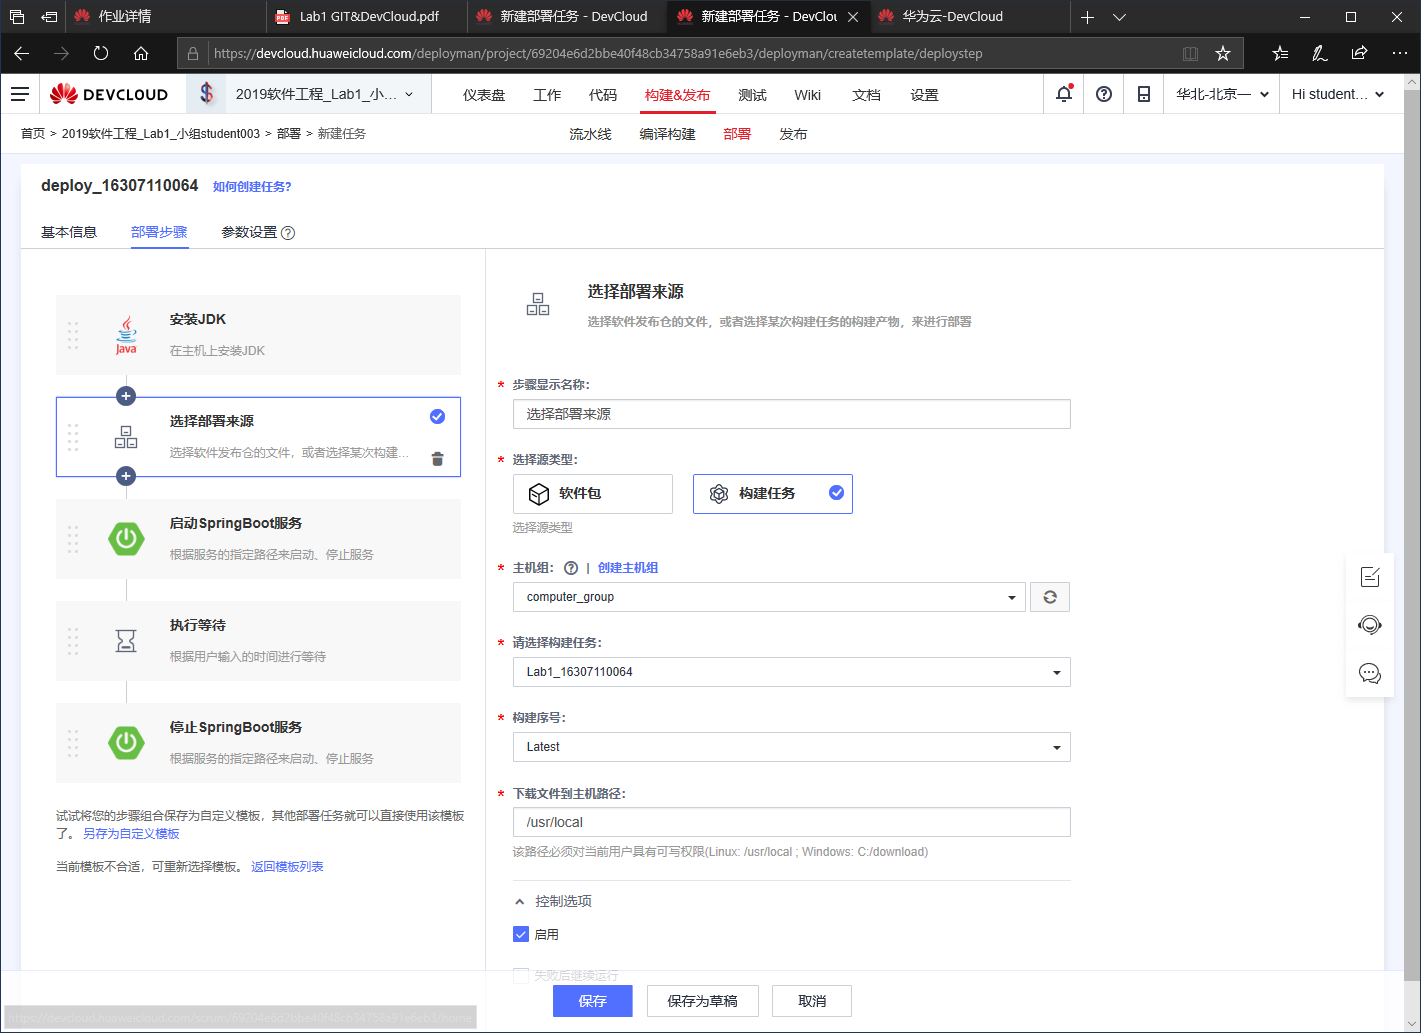
\includegraphics[width=12cm]{Figures/Capture6.png}
  \caption{Result of the adjusted deploy sequence}\label{9}
\end{figure}
\subsection{Configure startup service}
In the ``Start Spring Boot Service'' section, we should configure the start-up service at the absolute path \emph{/usr/local/lab1-0.0.1-SNAPSHOT.jar} and configure as the information given. The host should be the one we have created in the previous subsection. The result of the configured startup service is shown as the Figure \ref{10} below.
\begin{figure}
  \centering
  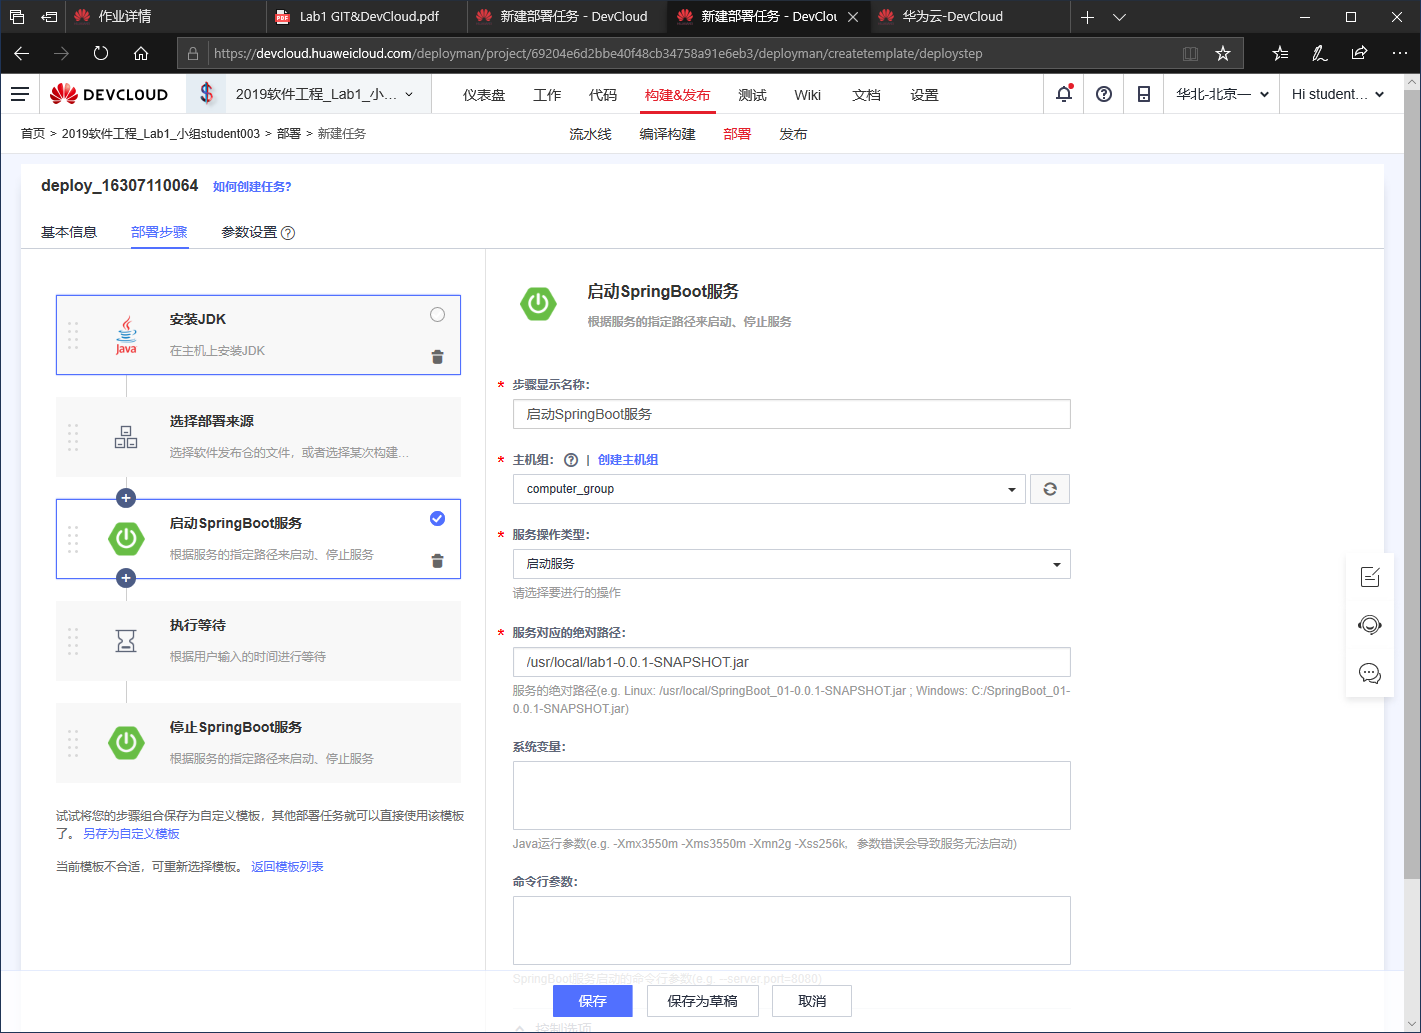
\includegraphics[width=12cm]{Figures/Capture7.png}
  \caption{Result of the configured startup service}\label{10}
\end{figure}
\subsection{Configure pending execution}
In the ``Configure pending execution'' section, we should create a 200 second pending time for us to visit our service. The result of the configured pending execution is shown as the Figure \ref{11} below.
\begin{figure}
  \centering
  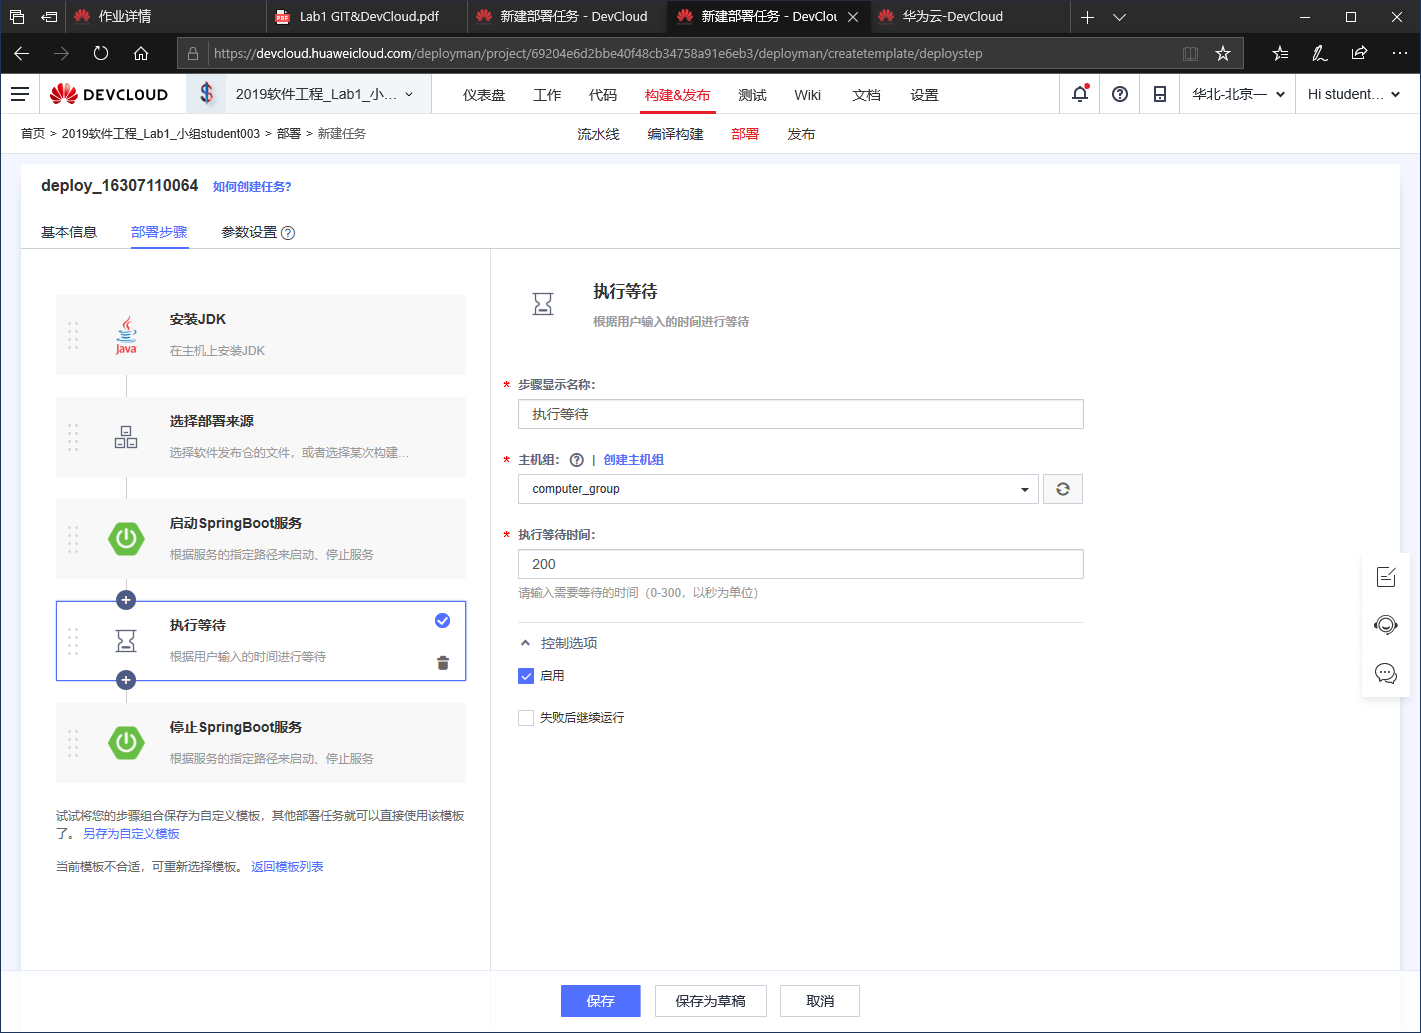
\includegraphics[width=12cm]{Figures/Capture8.png}
  \caption{Result of the configured pending execution}\label{11}
\end{figure}
\subsection{Configure stopping service}
In the ``Configure stopping service'' section, we should configure the stop service at the absolute path \emph{/usr/local/lab1-0.0.1-SNAPSHOT.jar} and configure as the information given. The host should be the one we have created in the previous subsection. The result of the configured stop service is shown as the Figure \ref{12} below.
\par
\begin{figure}
  \centering
  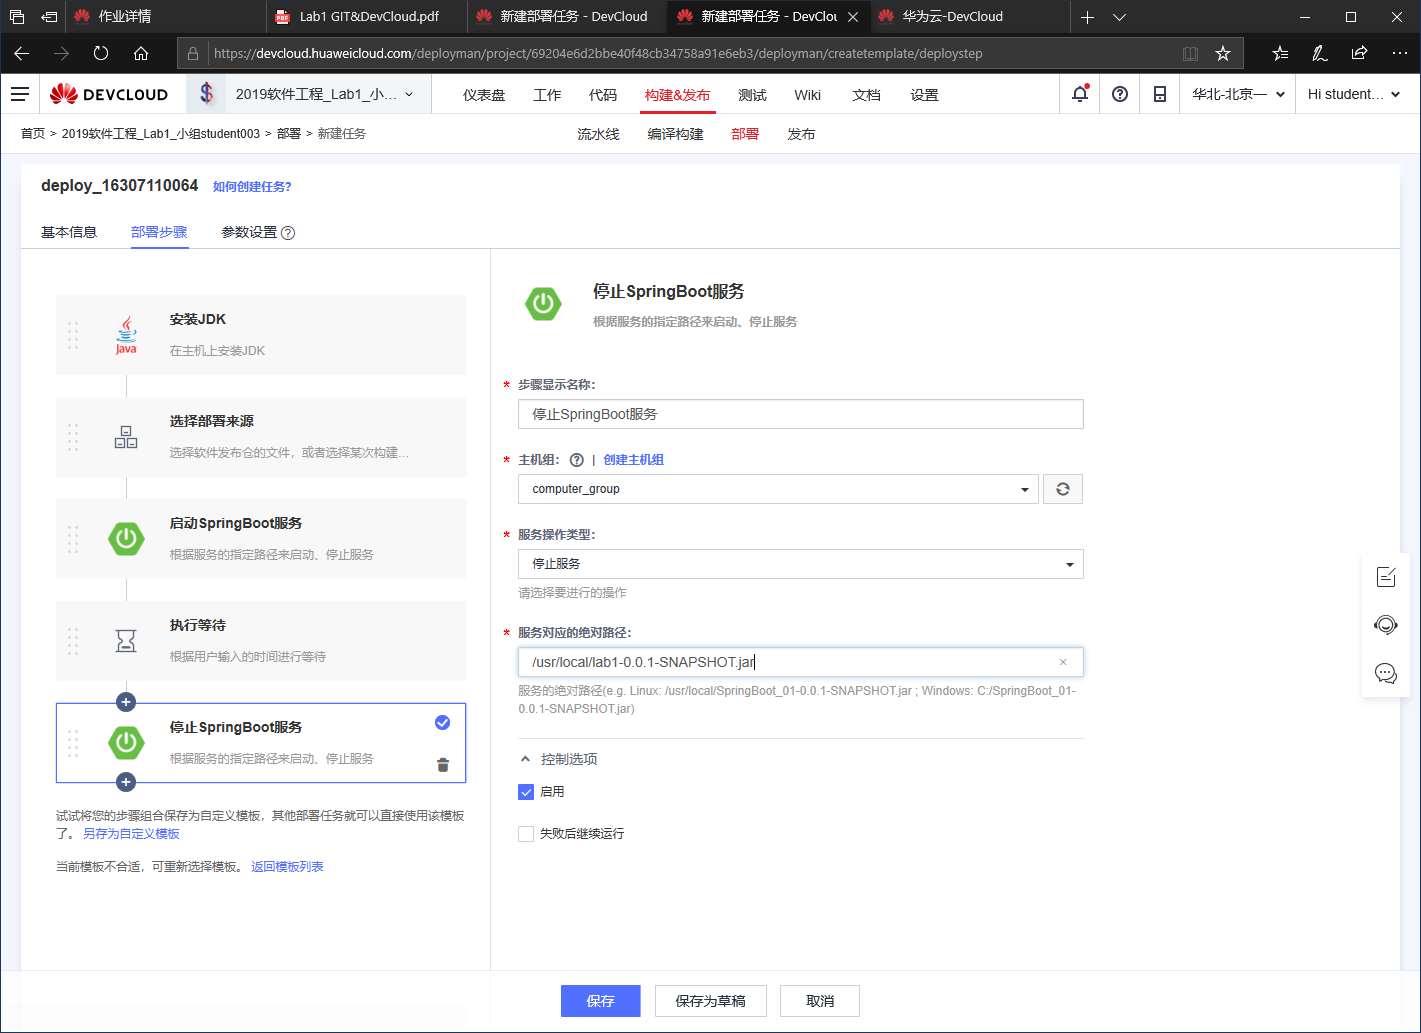
\includegraphics[width=12cm]{Figures/Capture9.png}
  \caption{Result of the configured startup service}\label{12}
\end{figure}
\par
\subsection{Start deployment}
As we choose to save and start the deployment process, we can observe the process of our project being deployed on the Huawei Dev Cloud.  The result of the start deployment process is shown as the Figure \ref{13} below.
\begin{figure}
  \centering
  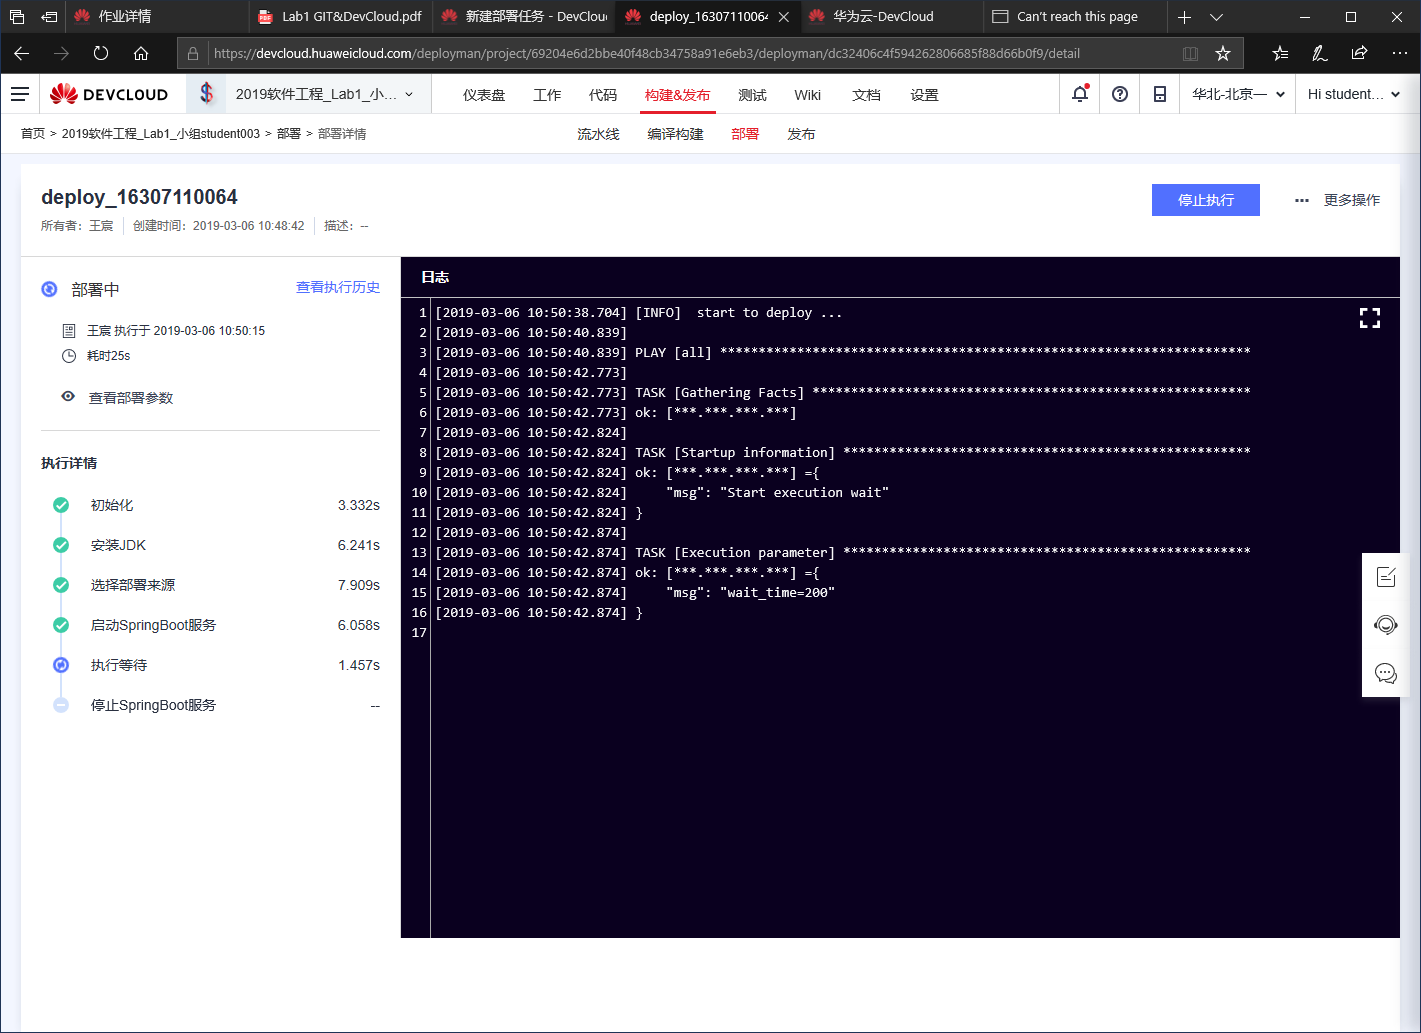
\includegraphics[width=12cm]{Figures/Capture10.png}
  \caption{Result of the start deployment process}\label{13}
\end{figure}
\subsection{Test the deployed application}
While our service is running, we can visit our service by the host IP address and the port number. The result of the test deployed application part is shown as the Figure \ref{14} below.
\begin{figure}
  \centering
  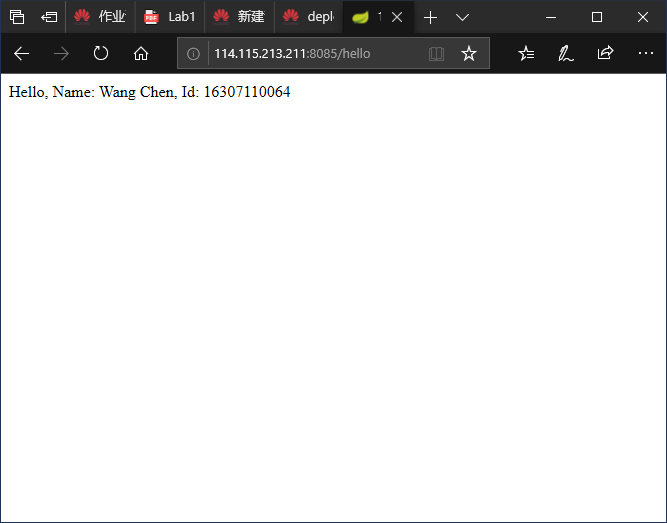
\includegraphics[width=12cm]{Figures/Capture11.png}
  \caption{Result of the test deployed application}\label{14}
\end{figure}
\chapter{Conclusion}
In this lab, I have experienced the entire life cycle of a project in software engineering. What has benefited me more is the process of exploring the new frameworks that I have never used before in the project. In addition, I am also enhanced by the convenience of the Huawei Cloud platform, which can integrate Code management, host management, web site distribution and deployment in simply one site. In the proceeding part of this lesson, I am sure to have more enact comprehension of the software development cycle and more details in software engineering.
\end{document} 